

\chapter{Basics}

In this background chapter, we review the statistical and probabilistic methodologies .
The goal of this chapter is to provide the basic information regarding Bayesian methods of machine learning used in the thesis. A good introduction to the field can be found in books of \cite{bishop2007pattern}, \cite{kruschke2014doing} and \cite{lee2014bayesian} . 

\section{Model Based Machine Learning}

Model based machine learning (MBML) is a new paradigm of machine learning, which can be called as the logical convergence between 2 related fields, statistics and machine learning. MBML the goal is to provide a framework which supports the creation of a wide range of models \cite{Bishop20120222}.

In traditional machine learning(SVM, Random Forest etc.) the approach is to map the problem onto a standard algorithm. Thus the algorithm is always fixed and the problem is modified to fit the algorithm.

Model based machine learning has a different take on the problem. Here the approach is to find the model which can represent the problem. The designed model is now used to generate a algorithm which will learn from the data. Thus MBML seeks to create a tailored algorithm for each problem. Such an approach makes the machine learning more flexible and better to understand/explain.

The framework emerged from an important convergence of three key ideas:
   \begin{itemize}
	\item the adoption of Bayesian methodologies for model learning.
	\item the use of graphical models, and
	\item the application of fast, deterministic, efficient and approximate inference algorithms
\end{itemize}

We give a short introduction to Bayesian model learning and graphical models. Inference algorithms is not covered, for a detailed discussion on inference algorithm please refer \cite{beal2003variational}, \cite{minka2001family}

\section{Bayesian Model Learning}

In MBML, models are used to represent the problem. Each problem in machine learning has a two parts: one a set of inputs called observed variables(input features and expected output); second a set of  quantities to be learned called latent unknown variables. In Bayesian modelling both these variables(observed and latent) are probabilities or probability distributions which are updated using Bayes theorem. 

Bayesian models are represented as probability distributions. Probability is used to quantify ``uncertainty" or ``Degree of belief". The models are initialized with some prior probabilities(beliefs). The observed data are used to update the prior beliefs to become posterior beliefs.

We can explain this with an example \cite{lee2014bayesian}. Assume you
are given a test that consists of 10 factual questions of equal difficulty. What we want to estimate is your ability, which we define as the rate $\theta$ with which you answer questions correctly. We cannot directly observe your ability $\theta$. All that we can observe is your score on the test. Before we do anything else (for example, before we start to look at your data) we need to specify our prior uncertainty with respect to your ability $\theta$. This uncertainty needs to be expressed as a probability distribution, called the ``prior distribution". In this case, keep in mind that $\theta$ can range from 0 to 1, and that we do not know anything about your familiarity with the topic or about the difficulty level of the questions. Then, a reasonable ``prior distribution,” denoted by $p(\theta)$, is one that assigns equalprobability to every value of $\theta$. This uniform distribution is shown by the dotted horizontal line in Figure \ref{fig: bayes}.

Now we consider your performance, and find that you answered 9
out of 10 questions correctly. After observing the data, the updated knowledge about $\theta$ is described by a \emph{posterior distribution}, denoted by $p(\theta | D)$. This distribution expresses the uncertainty about the value of $\theta$, quantifying the relative probability that each possible value is the true value.. Bayes rule specifies how we can combine the information from the data, that is how to determine the posterior distribution $p (\theta | D)$ using  the prior distribution $p(\theta)$ and the likelihood  $p (D | \theta)$ :
\begin{equation}
	p(\theta | D) = \frac{p(D | \theta) p(\theta)}{p(D)}
\end{equation}

The equation is often verbalized as :
\begin{equation}
	posterior = \frac{likelihood * prior}{marginal likelihood}
\end{equation}

We note here that the posterior distribution is a combination of the prior information we had and what we have learned from the data. 

\begin{figure}[htp]
\centering
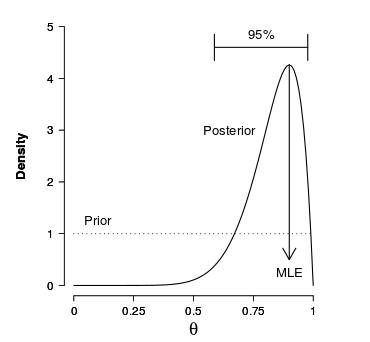
\includegraphics[width=0.5\textwidth]{images/bayes.png}
\caption[Bayesian parameter estimation]{Bayesian parameter estimation for rate parameter $\theta$
, after observing 9 correctresponses and 1 incorrect response. The mode of the posterior distribution for $\theta$ is 0.9, equal to the maximum likelihood estimate (MLE), and the 95\% credible interval extends from 0.59 to 0.98}
\label{fig: bayes}
\end{figure}


\section{Distributions }

The basic idea of Bayesian analysis is that quantifying the \emph{state of belief} or the \emph{state of uncertainty}, about the variables of interest. These variable(latent and observed) are always represented by probability distributions.  Probability distribution is just another name for a probability measure.  In this thesis we exhaustively use the Dirichlet, Categorical and Bernoulli distributions. 
 

\subsection*{Bernoulli distribution}
\todo[inline]{Explain}
Bernoulli distribution is used when there are a number of iterations of some activity, where each iteration (or observation) may turn out to be a ``success" or a ``failure". From the data on T observations, we want to estimate the probability of ``success"


\subsection*{Categorical distribution}
\todo[inline]{Explain}


\subsection*{Dirichlet distribution}
The Dirichlet distribution is part of the exponential family. It has finite dimensional sufficient statistics. It is conjugate to the multinomial and categorical distribution. 





\section{Probabilistic Graphical Models}

Probabilistic Graphical Models (PGM) is the formal lingua franca for probabilistic Bayesian modelling. PGM is a method to visualize complete and interpretable representation of a Bayesian probabilistic model. The nodes in the graph represent variables of the problem, and the edges connecting them represents dependencies. The graph structure is used to indicate dependencies between the variables, with children depending on their parents. The plates are used to indicate replication. We use the conventions of representing unobserved variables without shading and observed variables with shading.

Lets draw the PGM for the problem defined above. Beta distribution with parameters (1,1) can be selected as the prior distribution, while the ability can be represented using Bernoulli distribution. Thus the model is defined as 
\begin{equation}
	\theta \sim Beta(1,1) \\
	P(D|\theta) \sim Bernoulli(\theta)
\end{equation}

The graphical model can be shown as :

\begin{figure}[!h]
\centering


\tikz {
\centering
 % Define nodes
  \node[latent]                                 (theta) {$\theta$};
  \node[obs, below=of theta]                    (D)     {$D$}; 
  % Connect the nodes
  \edge {theta} {D};
  % plates
  \plate {location} {(D)} {n=0,....,9};
}
\caption[Graphical Model]{Graphical Model: Shaded node observed variable and non-shaded node is latent variable}
\end{figure}

\section{Probabilistic Programming Languages}

Probabilistic programming languages(PPL) are new languages developed to program probabilistic graphical models and to run inference in them. 
Until recently, Bayesian Model learning have been limited in scope, and have been hard to apply to many real-world applications. Probabilistic programming is a new approach using which one can construct Bayesian models faster and in a less error-prone way. 


\begin{figure}[htp]
\centering
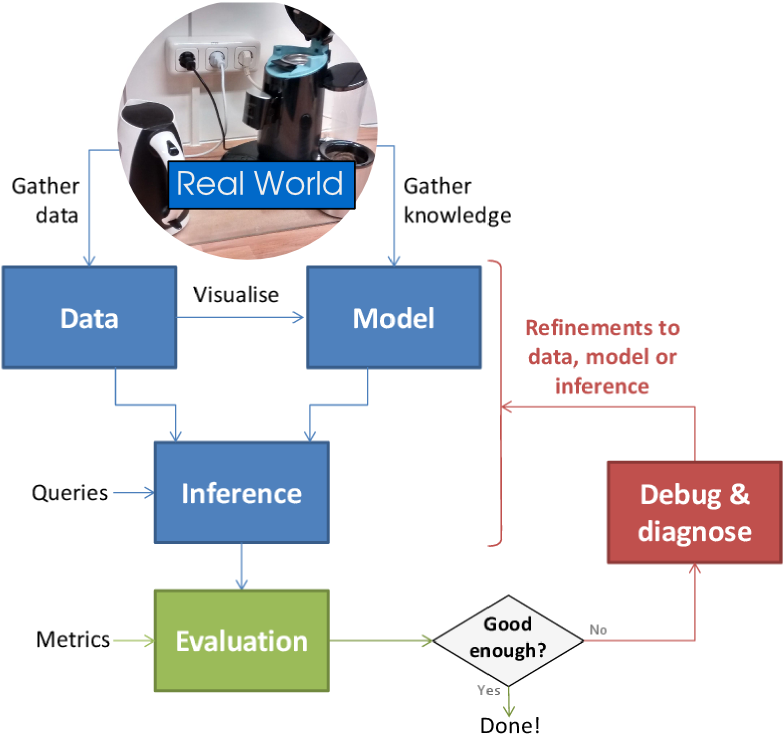
\includegraphics[width=0.5\textwidth]{pictures/Lifecycle.png}
\caption[Steps involved in probabilistic modelling ]{Steps involved in probabilistic modelling  \protect\footnotemark }
\label{}
\end{figure}

\footnotetext{\url{ http://www.mbmlbook.com/LifeCycle.html}}
\textbf{Probabilistic Programming} gives us a framework in which we can create any model, based on our assumptions of the process. The model is basically expressing the assumptions in a mathematical form. The assumptions are the number of variables in the model, the relation between these variables, changes in which variables affects which other variables. This model is then used to generate a problem specific algorithm which can be used to solve the machine learning problem in hand. 

\subsection*{Steps required in Probabilistic Modelling}
\label{sub:steps}
\begin{enumerate}
	\item \textbf{Gather data} to be used for training and evaluation.
    \item \textbf{Gather knowledge} required for model building.
    \item \textbf{Visualise} the data to understand it. This is useful also for gathering knowledge. After visualization the insight gained can be used for assumptions in model building.
    \item \textbf{Construct a model} based on the knowledge of the problem statement available and data visualization. 
    \item \textbf{Perform inference} using both the data and the constructed model. The variables of the model are tuned based on the data available. Predictions can be made to find out the knowledge gained by the model.
    \item \textbf{Evaluate} the performance of the model based on evaluation metric.
    \item \textbf{Diagnose} the model and the assumptions if the evaluation is below some acceptable range
    \item \textbf{Refine the system} by adapting different model structure, inference engine

\end{enumerate}
% subsection steps (end)


The separation of the model choices and the inference engine for generating machine algorithms have given rise to a new kind of programming language.
In the software framework you need to provide the description of your model and the selection of the inference engine, which internally produces the code for the machine learning algorithm.
Examples of software frameworks that implement the probabilistic modelling philosophy  include CHURCH \cite{goodman_church_2012}, Venture \cite{mansinghka_venture_2014}, PyMC3 \cite{salvatier_probabilistic_2015}, BayesPy \cite{luttinen_bayespy_2014} and Infer.net \cite{minka_2010}.

\subsection{PyMC3}

\textbf{PyMC3} is python module for Bayesian modelling. It provides intuitive model specification syntax for designing the models. The inference is primarily focussed on advanced Markov chain Monto Carlo fitting algorithms.


\subsection{BayesPy}

\textbf{BayesPy} provides tools to do Bayesian modelling. In BayesPy users construct their models, observes data and then runs inference. The inference engine present in BayesPy is variational Bayesian inference.

\subsection{WebPPL}

\textbf{WebPPL} is a javascript module for Bayesian modelling. The inference is using Markov chain Monto Carlo algorithms. Its particularly useful for doing learning inside web based database like MongoDB.
